%!TEX root = ../crimson_throne_book_main.tex
% 2015-06-20
The companions return to the pixie court to confront king Tirmando with the truth. They make Furian confess what happened to Oakenbrow's sister. The little fey sobs and cries bitter tears as he explains that he lost Mirala to the quicksand of the Mistmoors while playing with her there. The king and his entire court are shocked to learn of Furian's role in Oakenbrow quest for vengeance. With a heavy heart Tirmando accepts that he had best take to opportunity to parley with the centaur, even though he admits that it will be hard for him to negotiate with the archer who killed so many of his subjects. Still, he sees no other solution to this conflict, other than killing his attacker, which he obviously does not favor. He also tells Furian that he will have to pay for his involvement in this tragedy and - more importantly - for his silence afterwards.\\

Next the king turns his attention to the companion: he realizes that he made a deal with them, to tell them where they can find blood cap mushrooms. These red toadstools are rumored to grow in the Mistmoors, but no one dares to venture there ... except for little Furian, it seems. As a first step on his path to redemption the king order the distraught little fey to accompany the companions to the swamps, a quest that Furian clearly doesn't like.\\

On their way south Furian tells the heroes more about the cursed moors. Hundreds of years ago it was the site of a huge battle between two human armies. Since that time the ghosts of the dead roam there, so the place was declared a {\itshape forbidden zone} . The pixie king had the Mist Lake flood the area, turning it into a swamp, so no one would go there anymore. Doubting the stories of old, Furian and Mirala tempted fate and went to the moors to see for themselves how dangerous they really were. The pixie has regretted this decision every second since Mirala drowned. The Mistmoors truly deserve their name, as they are clouded in eternal mist. The companions find no dry path through the swamp and before they know it they are up to their knees in murky waters. Quint pulls out his {\itshape wand of featherstep} to have everyone move more freely through the difficult terrain. Sjo takes Puk on his shoulders, since the halfling is too short to walk here, while Spyder is reduced to jumping and swimming. Furian removes his cloak to reveal his wings and takes to the air. Sjo sends him up to scout the area from above, but the pixie has a hard time relocating the heroes when he descends again, serving only to increase his fear. He testifies that the entire swamps are covered in a thick veil of mist. After twenty minutes the waters become even deeper and suddenly Quint can't free his feet anymore. He starts sinking slowly and his friends have to throw him a rope to pull him out. Furian explains that they have already travelled deeper into the moors than he and Mirala did, but still there is no sign of the red mushrooms. Then Sjo picks up strange whispers, but his friends claim not to have heard anything. A minute later Balian thinks he sees a shadow move in the mists; Quint calls out and is answered by a whispering sound coming from behind him, but again the others say they haven't heard a thing. Then Furian grabs his head: "They are here! Can't you hear them?" The scared pixie quickly turns invisible, as the mists seem to sigh from all sides.\\

Next a fearsome warcry resounds in Shoanti: "For the Shadde-Quah! Kill them all! Kill them all!" Four shapes tear themselves from the fog, seeming to be made of white smoke themselves. These must be the ghosts of Shoanti barbarians who fell here, seeking to destroy the Korvosan intruders. Sjo pulls out the amulet he recovered from the Shoanti tumulus outside of Harse and shouts that he is a {\itshape nalharest} , friend of the Shoanti, while Quint starts a Shoanti song to calm the attackers. These attempts do not sway the enraged assailants from attacking, although the incorporeal barbarians focus their attention on the other companions: Balian and Puk. Balian gets hit several times by a misty battleaxe, while Puk's armor proves no defense for one ghost's corrupting touch. Balian's greatsword cleaves through the opponents, tearing away wisps of their ghostly bodies. When Sjo and Quint give up their attempts to reason with the aggressors and join the fight, they get targeted as well. Quint can hurt the ghosts with his  {\itshape wand of magic missiles} , but realizes that just two magical arrows per attack will not suffice to take down the opponents quickly. He summons  {\itshape mirror images} of himself and jumps into melee with his short sword instead. Sjo heals Puk's and Balian's worst wounds and swings his morningstar at the barbarians. He ends up striking the 'killing' blow on two ghosts, while Puk and Balian slay the other two. Our friends start to wonder if it is actually a good idea to travel the swamps blindly. Still they press on. Puk climbs one of the large mangrove like trees, only to learn that he can't make out anything in the mist. He finds no blood cap mushrooms in the tree either. As he comes back down, Balian's attention is drawn by soft splashes of water. While the ranger draws his blade, a boat appears with three lizardmen. The one in front hurls a javelin at Balian, but fails to hit him. The trio of scaly creatures is clearly outmatched by the heroes and only moments later they are defeated. Quint notices that two of the dead lizardmen wear necklaces made of flowers, much like the ones they found in Mirala's cave or around Furian's neck. The pixie also recognizes the handiwork of his centaur playmate and is filled with hope that his best friend is still alive. The companions take the lizardmen's boat and Balian sits down at the oars, demonstrating his skill at rowing which he developed as a galley slave. He chooses the direction the scaly hunters came from, gliding slowly over the muddy water. His instincts guide him well and half an hour later he picks up the beating of a drum. He steers the boat in the direction of the noise. Suddenly the mists clear and reveal\hyperref[fig:Approaching-the-lizardmen-village-540871537]{ a small settlement of pile dwellings } . \\

\begin{figure}[h]
	\centering
	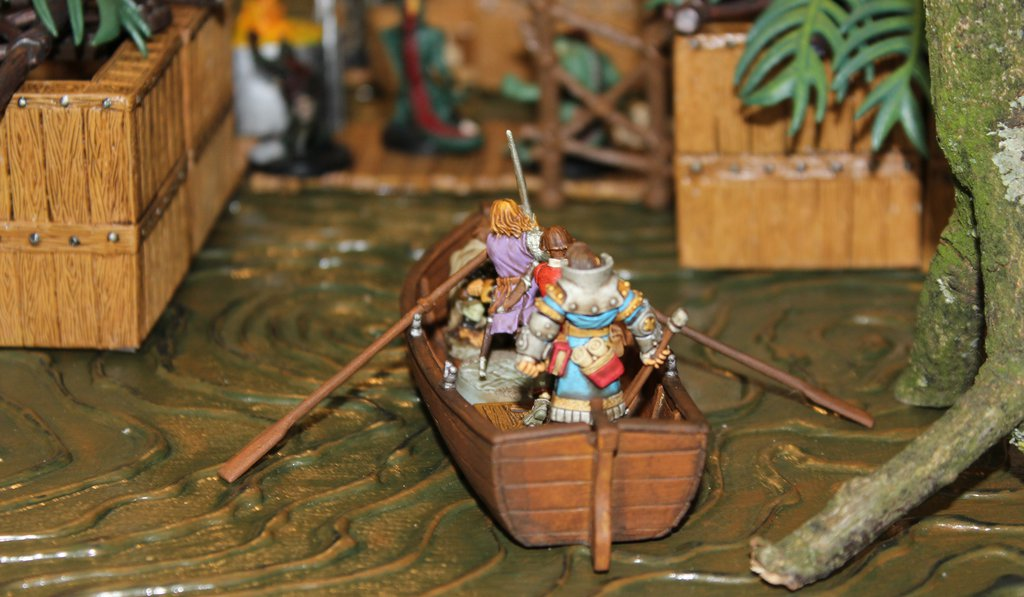
\includegraphics[width=0.39\textwidth]{images/Approaching-the-lizardmen-village-540871537.jpg}
	\caption{Approaching the lizardmen village}
	\label{fig:Approaching-the-lizardmen-village-540871537}
\end{figure}

